\documentclass[pdf, autumn, slideColor, nocolorBG]{prosper}
\usepackage{verbatim}
\usepackage{color}
\usepackage{hyperref}
\usepackage{biblatex}
\usepackage{subfig}
\usepackage{tikz}
\usetikzlibrary{shapes,arrows}


%General Short-Cut Commands
\newcommand{\superscript}[1]{\ensuremath{^{\textrm{#1}}}}
\newcommand{\subscript}[1]{\ensuremath{_{\textrm{#1}}}}
\newcommand{\nuc}[2]{\superscript{#2}{#1}}
\newcommand{\FigCaption}[1]{\begin{center}{\tiny{#1}}\end{center}}

%Commands for this document...
\newcommand{\Red}[1]{\textcolor{red}{#1}}


% Bibliography
\bibliography{library}{}


% Presentation information
\title{Fuel Cycle Covariance of Plutonium and Americium Separations to Repository Capacity using Information Theoretic Measures}
\subtitle{GLOBAL 2011 - December 15\superscript{th}, 2011 - Makuhari, Japan}
\author{Anthony Scopatz\superscript{1}, Jun Li\superscript{2}, Erich Schneider\superscript{3}, Man-Sung Yim\superscript{4}}
\email{scopatz@flash.uchicago.edu}
\institution{\tiny
\superscript{1}The University of Chicago; 
\superscript{2}University of North Carolina at Chapel Hil\\
\superscript{3}The University of Texas at Austin; 
\superscript{4}KAIST
}

\slideCaption{Scopatz - GLOBAL 2011}

\begin{document}

% make the title slide
\maketitle


% Motivation
\overlays{5}{
\begin{slide}{Motivation}
\FromSlide{1}
\begin{itemize}
    \item Many nuclear fuel cycle simulations are formulated on premade base-case scenarios:

\FromSlide{2}
    \begin{center}
    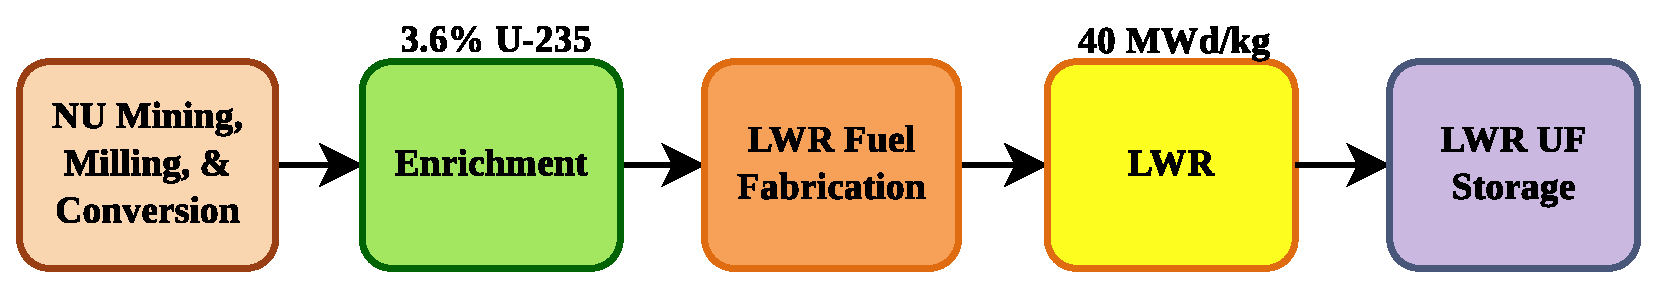
\includegraphics[scale=0.25]{figs/OnceThrough.eps}
    \end{center}

\FromSlide{3}
    \item These base cases are very well studied.

\FromSlide{4}
    \item However, what is \textbf{\textit{not}} well known is 
        how these sample scenarios are affected by perturbations to their 
        initial physical parameters.
            
\FromSlide{1}
\end{itemize}

\FromSlide{5}
\begin{center}
``\textit{Do our parameter choices really give us the `best' solution?}''
\end{center}

\end{slide}}




% Motivation
\overlays{5}{
\begin{slide}{Motivation}
\FromSlide{1}
\begin{itemize}
    \item Many fuel cycle sensitivity studies focus on linear, 
        1D parameter sweeps from base case scenarios.

\FromSlide{2}
    \item However, a set of fuel cycle component models which 
        preserve basic physics has been developed. 

\FromSlide{3}
    \item This suite largely focused on a one-energy 
        group reactor model [1] and a deep geologic
        repository model [2].

\FromSlide{4}
    \item These essential physics models were used to extend the 
        fuel cycle sensitivity studies to simelateously perturb 
        many continuous variables.  

\FromSlide{5}
    \item Such studies require a stochastic driving mechanism
        to run.  Moreover, they require entropy-based measures to
        analyze.

\FromSlide{1}
\end{itemize}
\end{slide}}





% Fuel Cycle
\overlays{2}{
\begin{slide}{Fuel Cycle}
\FromSlide{1}
\begin{itemize}
    \item The essential physics models were
        used to study a Fast Reactor (FR), Light
        Water Reactor (LWR) symbiotic scenario 
        analogous to Scheme 3a of a 2006 OECD report [3].
\end{itemize}

\FromSlide{2}
\setcounter{figure}{0}
\begin{center}
\begin{figure}
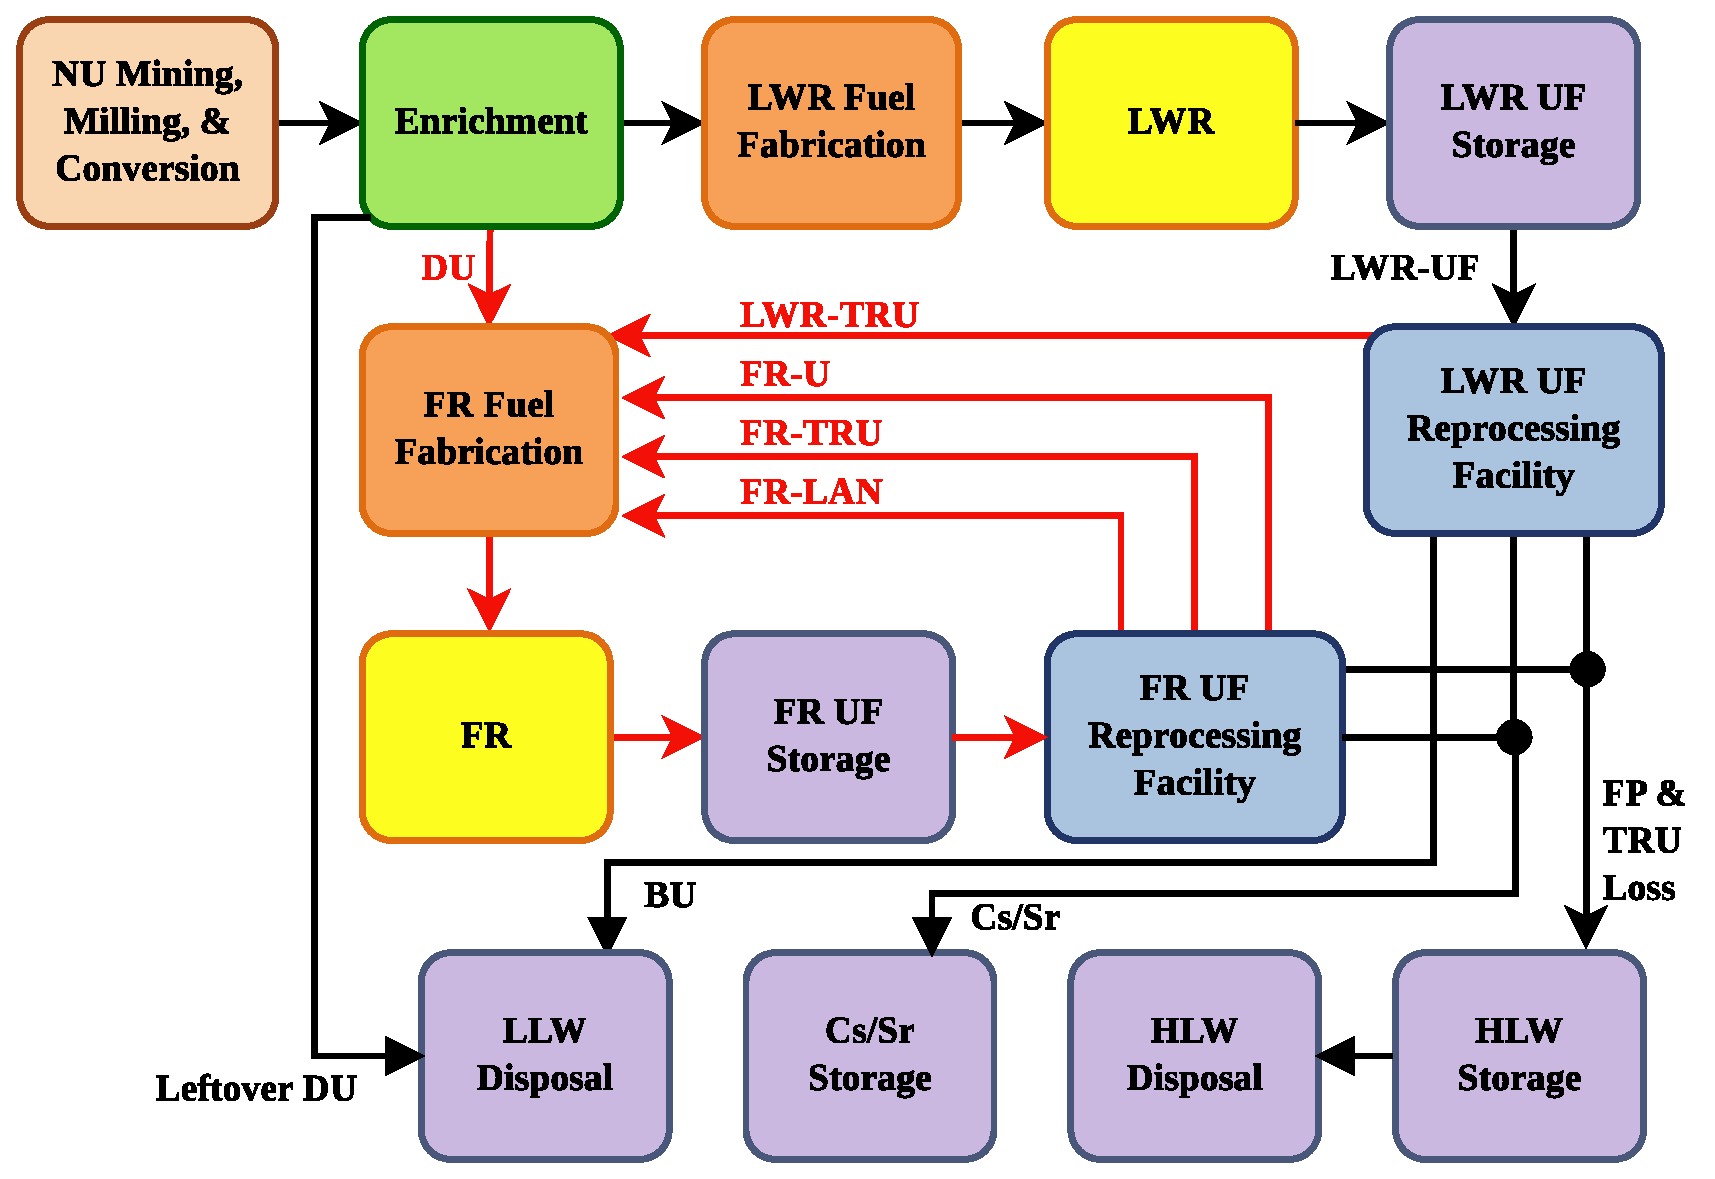
\includegraphics[scale=0.2]{figs/LWR_FR_FC.eps}
\caption{LWR-FR Fuel Cycle}
\end{figure}
\end{center}
\end{slide}}




% Fuel Cycle
\overlays{3}{
\begin{slide}{Fuel Cycle}
\FromSlide{1}
\small
With perturbable components, over 30 independent physical 
parameters may be adjusted in the fuel cycle.
\FromSlide{2}
\setcounter{figure}{1}
\begin{figure}
\begin{center}
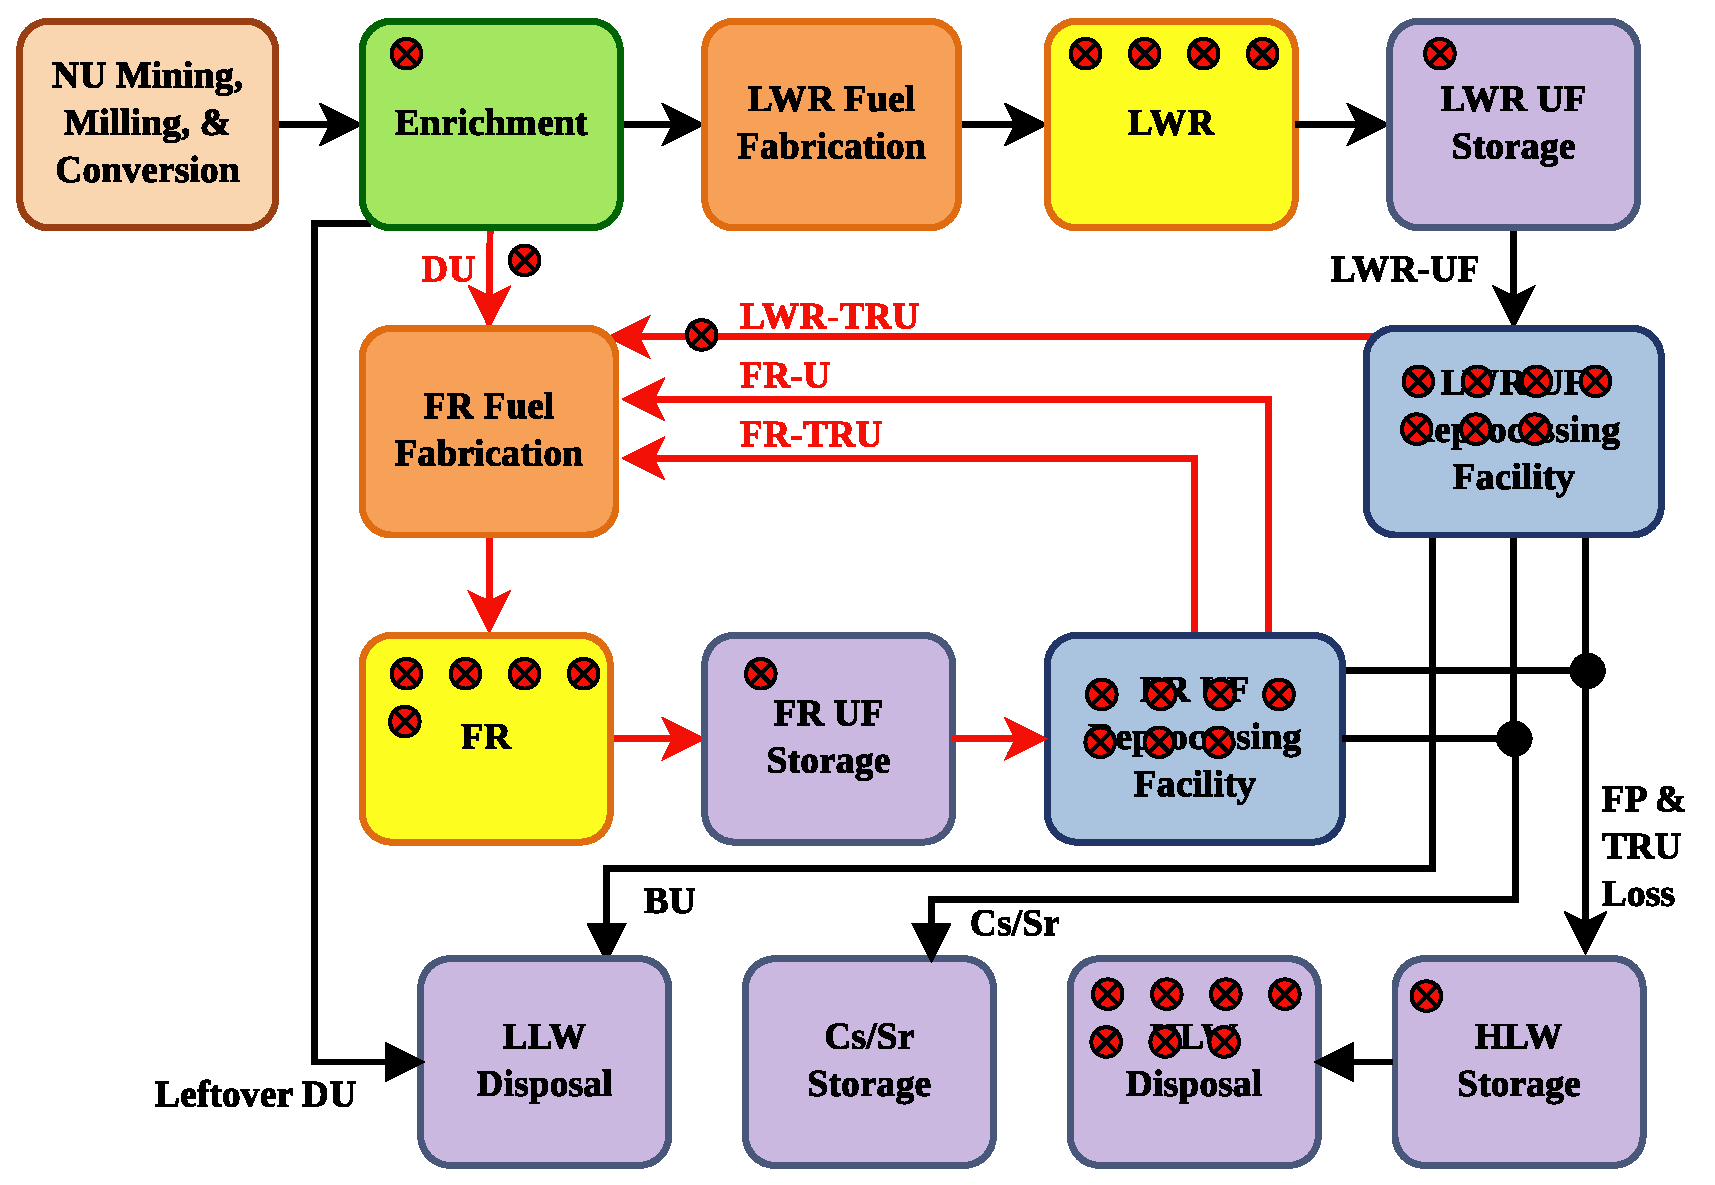
\includegraphics[scale=0.2]{figs/LWR_FR_FC_knobs.eps}
\caption{LWR-FR Cycle with Parameters}
\end{center}
\end{figure}
\FromSlide{3}
\small
Sensitivity results are computed from equilibrium values derived from 
a full treatment of the preceding, transient cycles.
\end{slide}}




% Base Case Parameter Definition
\begin{slide}{Base Case Parameter Definition}
\tiny
\begin{center}
\begin{tabular}{|l||c|c|}
\hline
\textbf{Input Parameter $x$} & \textbf{Value} & \textbf{Units} \\
\hline
LWR Burnup & 50.0 & MWd/kgIHM \\
\hline
LWR Fuel to Moderator Ratio & 0.301 & \\
\hline
LWR UF Storage Time & 60 & years \\
\hline
SE of U from LWR UF & 0.999 & \\
\hline
SE of NP from LWR UF & 0.999 & \\
\hline
SE of PU from LWR UF & 0.999 & \\
\hline
SE of AM from LWR UF & 0.999 & \\
\hline
SE of CM from LWR UF & 0.999 & \\
\hline
SE of CS from LWR UF & 0.999 & \\
\hline
SE of SR from LWR UF & 0.999 & \\
\hline
FR Burnup & 140.0 & MWd/kgIHM \\
\hline
FR TRU Conversion Ratio & 0.50 & \\
\hline
Max Fraction of Lanthanide in FR Fuel & 0.0005 & Atoms/TRU Atom \\
\hline
FR UF Storage Time & 3 & years \\
\hline
Storage Before Disposal & 50 & years \\
\hline
\end{tabular}
\end{center}
\end{slide}



% Base Case Parameter Definition
\begin{slide}{Base Case Parameter Definition}
\tiny
\begin{center}
\begin{tabular}{|l||c|c|}
\hline
\textbf{Input Parameter $x$} & \textbf{Value} & \textbf{Units} \\
\hline
SE of U from FR UF & 0.999 & \\
\hline
SE of NP from FR UF & 0.999 & \\
\hline
SE of PU from FR UF & 0.999 & \\
\hline
SE of AM from FR UF & 0.999 & \\
\hline
SE of CM from FR UF & 0.999 & \\
\hline
SE of CS from FR UF & 0.999 & \\
\hline
SE of SR from FR UF & 0.999 & \\
\hline
Density of Host Rock & 2580 & kg/m\superscript{3} \\
\hline
Specific Heat of Host Rock & 840 & J/kg-K \\
\hline
Thermal Conductivity of Host Rock & 1.626 & W/m-K \\
\hline
Heat Loss Factor During Ventilation  & 0.7 & \\
\hline
Drift diameter & 5.5 & m \\
\hline
Ventilation System On Time & 50 & years \\
\hline
Ambient Environment Temperature & 20 & C \\
\hline
Distance Between Drifts & 81 & m \\
\hline
\end{tabular}
\end{center}
\end{slide}






% Fuel Cycle Benchmark
\begin{slide}{Fuel Cycle Base Case Benchmark}
\tiny
\begin{center}
\begin{tabular}{|l||c||c|c||c|c|}
\hline
\textbf{Scheme 3a}     & \textbf{NEA [3]} & \textbf{Model\superscript{1}} & \textbf{\% Diff} & \textbf{Model\superscript{2}} & \textbf{\% Diff} \\
\hline
Electricity Share: LWR & 0.632       & 0.619459             & -2.0244 & 0.634907             & +0.4579 \\
\hline
Electricity Share: FR  & 0.368       & 0.380541             & +3.2955 & 0.365093             & -0.7962 \\
\hline
FR UF: U               & 0.698       & 0.713806             & +2.2143 & 0.715224             & +2.4082 \\
\hline
FR UF: NP              & 0.0065      & 0.00661961           & +1.8070 & 0.00685174           & +5.1335 \\
\hline
FR UF: PU              & 0.266       & 0.248059             & -7.2327 & 0.248319             & -7.1204 \\
\hline
FR UF: AM              & 0.02        & 0.0226796            & 11.8152 & 0.0217317            & +7.9687 \\
\hline
FR UF: CM              & 0.0098      & 0.00883517           & -10.920 & 0.00787319           & -24.4730\\
\hline
HLW: U                 & 0.013324    & 0.0132681            & -0.4213 & 0.0134448            & +0.8984 \\
\hline
HLW: NP                & 2.26542E-05 & 2.4079E-05           & +5.9173 & 2.41083E-05          & +6.0316 \\
\hline
HLW: PU                & 0.000704797 & 0.000658893          & -6.9668 & 0.000632361          & -11.4548\\
\hline
HLW: AM                & 5.03426E-05 & 5.63068E-05          & 10.5923 & 5.12344E-05          & +1.7405 \\
\hline
HLW: CM                & 2.18151E-05 & 1.99031E-05          & -9.6068 & 1.67094E-05          & -30.5563\\
\hline
HLW: FP                & 0.985876    & 0.985973             & +0.0098 & 0.985831             & -0.0046 \\
\hline
\end{tabular}
\end{center}

1: Model with initial LWR \nuc{U}{235} enrichment of 4.2 w/o. 

2: Model with LWR discharge burnup of 50 MWd/kg.
\end{slide}









% Contingency Table Methodology
\overlays{4}{
\begin{slide}{Contingency Table Methodology}
\FromSlide{1}
\begin{itemize}
    \item Here, the system-wide impact of physical parameter perturbations is quantified.

\FromSlide{2}
    \item This is done by performing \textbf{Contingency Table} analysis for each parameter
        to the \underline{repository} \underline{capacity} response.  

\FromSlide{3}
    \item Denote fuel cycle responses as $R$ [MTHM/Rep.] for $x$ \& $y$ input parameters.

\FromSlide{4}
    \item \textbf{\underline{Goal:}} Determine \textit{covariance} 
        pairs of inputs to the response in a manner that is independent of:
        \begin{itemize}
            \item the form of the response to the input $R(x,y)$
            \item and any base-case set of initial inputs.
        \end{itemize}

\FromSlide{1}
\end{itemize}
\end{slide}}






% Contingency Table Methodology
\begin{slide}{Contingency Table Methodology}
\begin{center}
\begin{figure}
\caption{Monte Carlo Methodology \& Analysis}
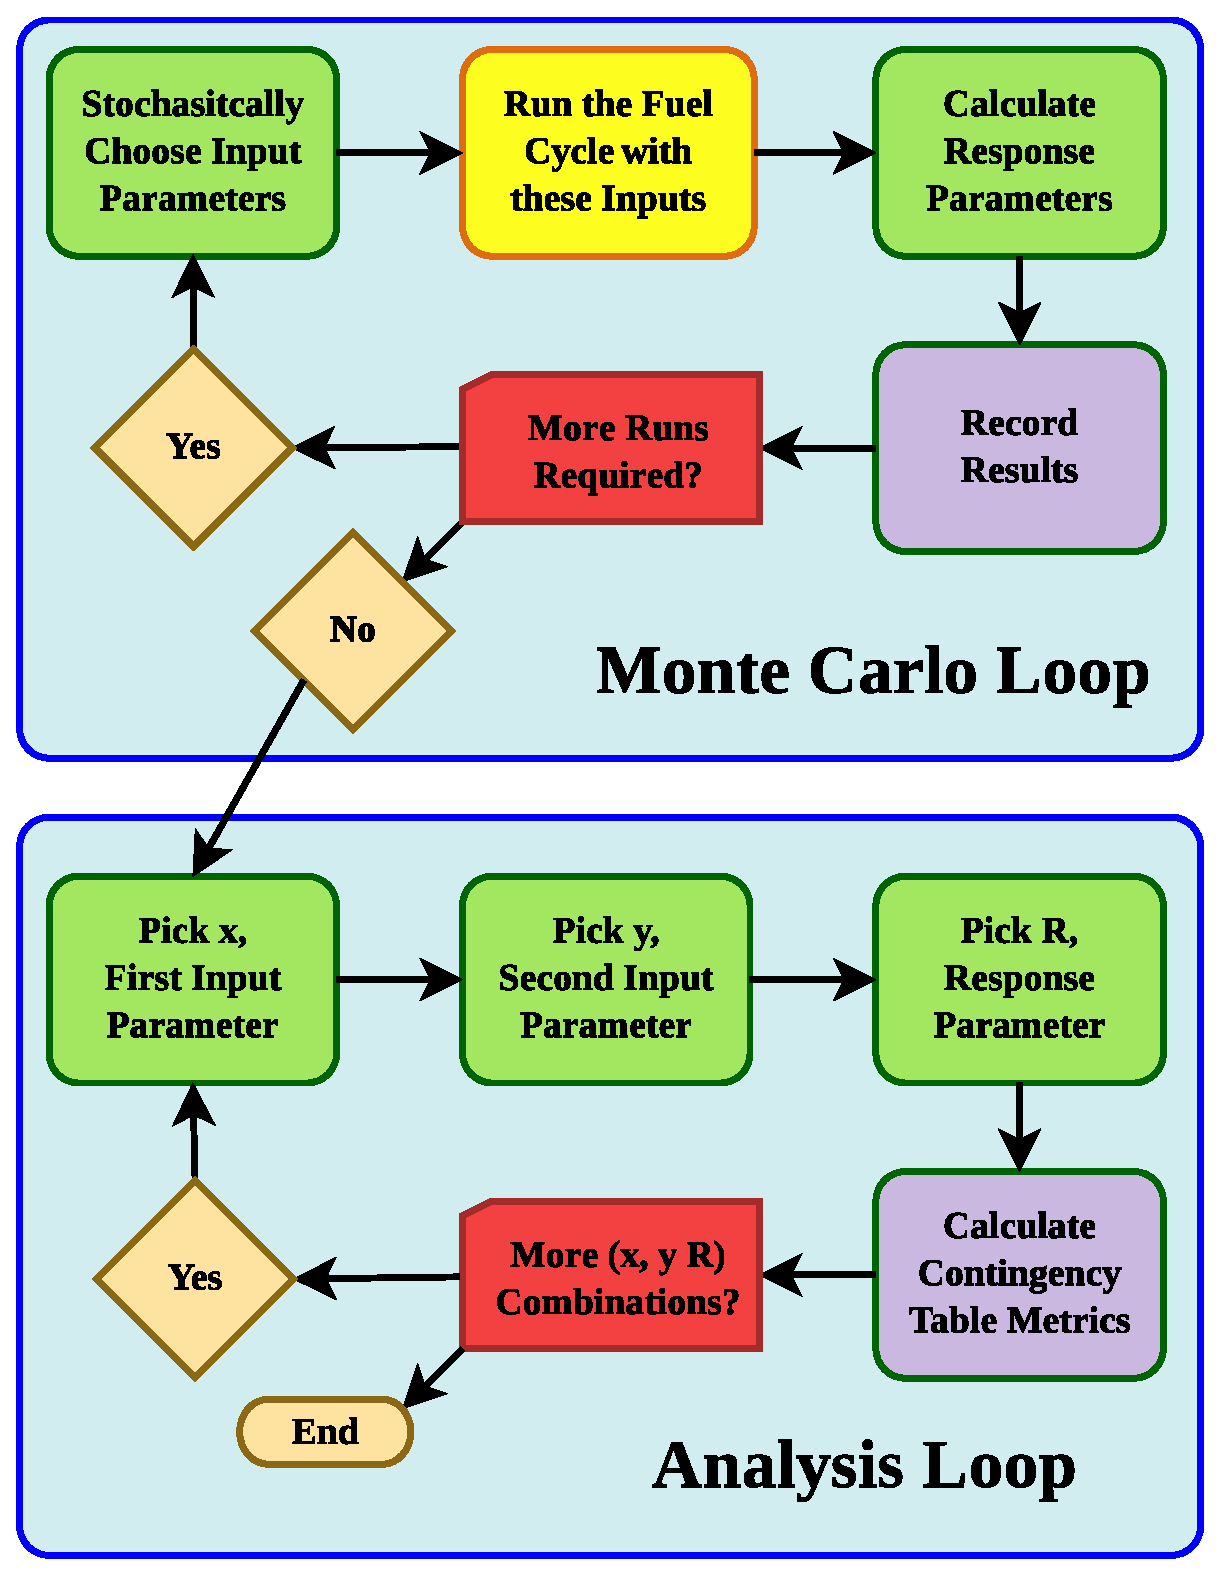
\includegraphics[scale=0.25]{figs/MonteCarloMethodology.eps}
\end{figure}
\end{center}
\end{slide}





% Input Parameter Definition
\begin{slide}{Input Parameter Definition}
\tiny
\begin{center}
\begin{tabular}{|l||c|c|c|c|}
\hline
\textbf{Input Parameter $x$} & \textbf{Min} & \textbf{Max} & \textbf{Units} & \textbf{Sample Type}\\
\hline
LWR Burnup Level & 30.0 & 80.0 & MWd/kgIHM & linear \\
\hline
LWR Fuel to Moderator Ratio & 0.28 & 0.36 & & linear \\
\hline
LWR SNF Storage Time & 3 & 30 & years & linear \\
\hline
SE of U from LWR UF & 0.99 & 0.9999 & & nines \\
\hline
SE of NP from LWR UF & 0.9 & 0.9999 & & nines \\
\hline
SE of PU from LWR UF & 0.9 & 0.9999 & & nines \\
\hline
SE of AM from LWR UF & 0.9 & 0.9999 & & nines \\
\hline
SE of CM from LWR UF & 0.9 & 0.9999 & & nines \\
\hline
SE of CS from LWR UF & 0.9 & 0.9999 & & nines \\
\hline
SE of SR from LWR UF & 0.9 & 0.9999 & & nines \\
\hline
FR Burnup Level & 100.0 & 200.0 & MWd/kgIHM & linear\\
\hline
FR TRU Conversion Ratio & 0.25 & 0.95 & & linear \\
\hline
Max Fraction of Lanthanide in FR Fuel & 0.0001 & 0.005 & Atoms/TRU Atom & linear \\
\hline
FR UF Storage Time & 3 & 30 & years & linear \\
\hline
Storage Before Disposal & 1 & 300 & years & log \\
\hline
\end{tabular}
\end{center}
\end{slide}

%Input Parameter Definition
\begin{slide}{Input Parameter Definition}
\tiny
\begin{center}
\begin{tabular}{|l||c|c|c|c|}
\hline
\textbf{Input Parameter $x$} & \textbf{Min} & \textbf{Max} & \textbf{Units} & \textbf{Sample Type}\\
\hline
SE of U from FR UF & 0.99 & 0.9999 & & nines \\
\hline
SE of NP from FR UF & 0.9 & 0.9999 & & nines \\
\hline
SE of PU from FR UF & 0.9 & 0.9999 & & nines \\
\hline
SE of AM from FR UF & 0.9 & 0.9999 & & nines \\
\hline
SE of CM from FR UF & 0.9 & 0.9999 & & nines \\
\hline
SE of CS from FR UF & 0.9 & 0.9999 & & nines \\
\hline
SE of SR from FR UF & 0.9 & 0.9999 & & nines \\
\hline
Density of Host Rock & 2317 & 2869 & kg/m\superscript{3} & linear \\
\hline
Specific Heat of Host Rock & 590 & 1270 & J/kg-K & linear \\
\hline
Thermal Conductivity of Host Rock & 1.9204 & 3.2856 & W/m-K & linear \\
\hline
Heat Loss Factor During Ventilation  & 0.806 & 0.914 & & linear \\
\hline
Drift diameter & 4.5 & 6.5 & m & linear \\
\hline
Ventilation System On Time & 10 & 300 & years & log \\
\hline
Ambient Environment Temperature & 12.82 & 32.82 & C & linear \\
\hline
Distance Between Drifts & 56 & 106 & m & linear \\
\hline
\end{tabular}
\end{center}
\end{slide}






% Contingency Table Methodology
\overlays{5}{
\begin{slide}{Contingency Table Methodology}
\FromSlide{1}
\begin{itemize}
    \item Before attempting to comprehend the subtleties of a 30+ dimensional surface,  
        prudence demands a check to see if all 30 variables are \textit{really} needed...

\FromSlide{2}
    \begin{itemize}
        \item (Hint: probably not!)
    \end{itemize}

\FromSlide{3}
    \item Previous studies explored the quantitative ranking of \emph{associations} 
        of each input parameters to the response [4].

\FromSlide{4}
    \item Here, the pairs of input parameters are ranked based on their
    \emph{covariance} to the response.  

\FromSlide{5}
    \item These rankings are obtained by borrowing an analysis tool that is often 
        used in Biology: \underline{Contingency Tables}.

\FromSlide{1}
\end{itemize}
\end{slide}}



% Contingency Tables
\overlays{3}{
\begin{slide}{Contingency Tables}
\FromSlide{1}
The $2\times 2$ table is most common:
\setcounter{table}{4}
\begin{center}
\begin{table}
\caption{Hair Color to Sex Contingency Table}
\begin{tabular}{|l||c|c||c|}
\hline
       & Blonde & Brunette & Totals \\
\hline
Female & 18     & 17       & 35 \\
\hline
Male   & 11     & 14       & 25 \\
\hline
Totals & 29     & 31       & 60 \\
\hline
\end{tabular}
\end{table}
\end{center} 

\FromSlide{2}
\vspace{0.5cm}
But doesn't this approach ignore the underlying biology?

\FromSlide{3}
\vspace{0.5cm}
\raggedleft{\LARGE \textit{Yes!}}
\end{slide}}



% Contingency Tables
\overlays{6}{
\begin{slide}{Contingency Tables}
\begin{center}
\onlySlide*{1}{
\includegraphics[scale=0.125]{figs/CTBlackBox/CTBlackBox01.eps}}

\onlySlide*{2}{
\includegraphics[scale=0.125]{figs/CTBlackBox/CTBlackBox02.eps}}

\onlySlide*{3}{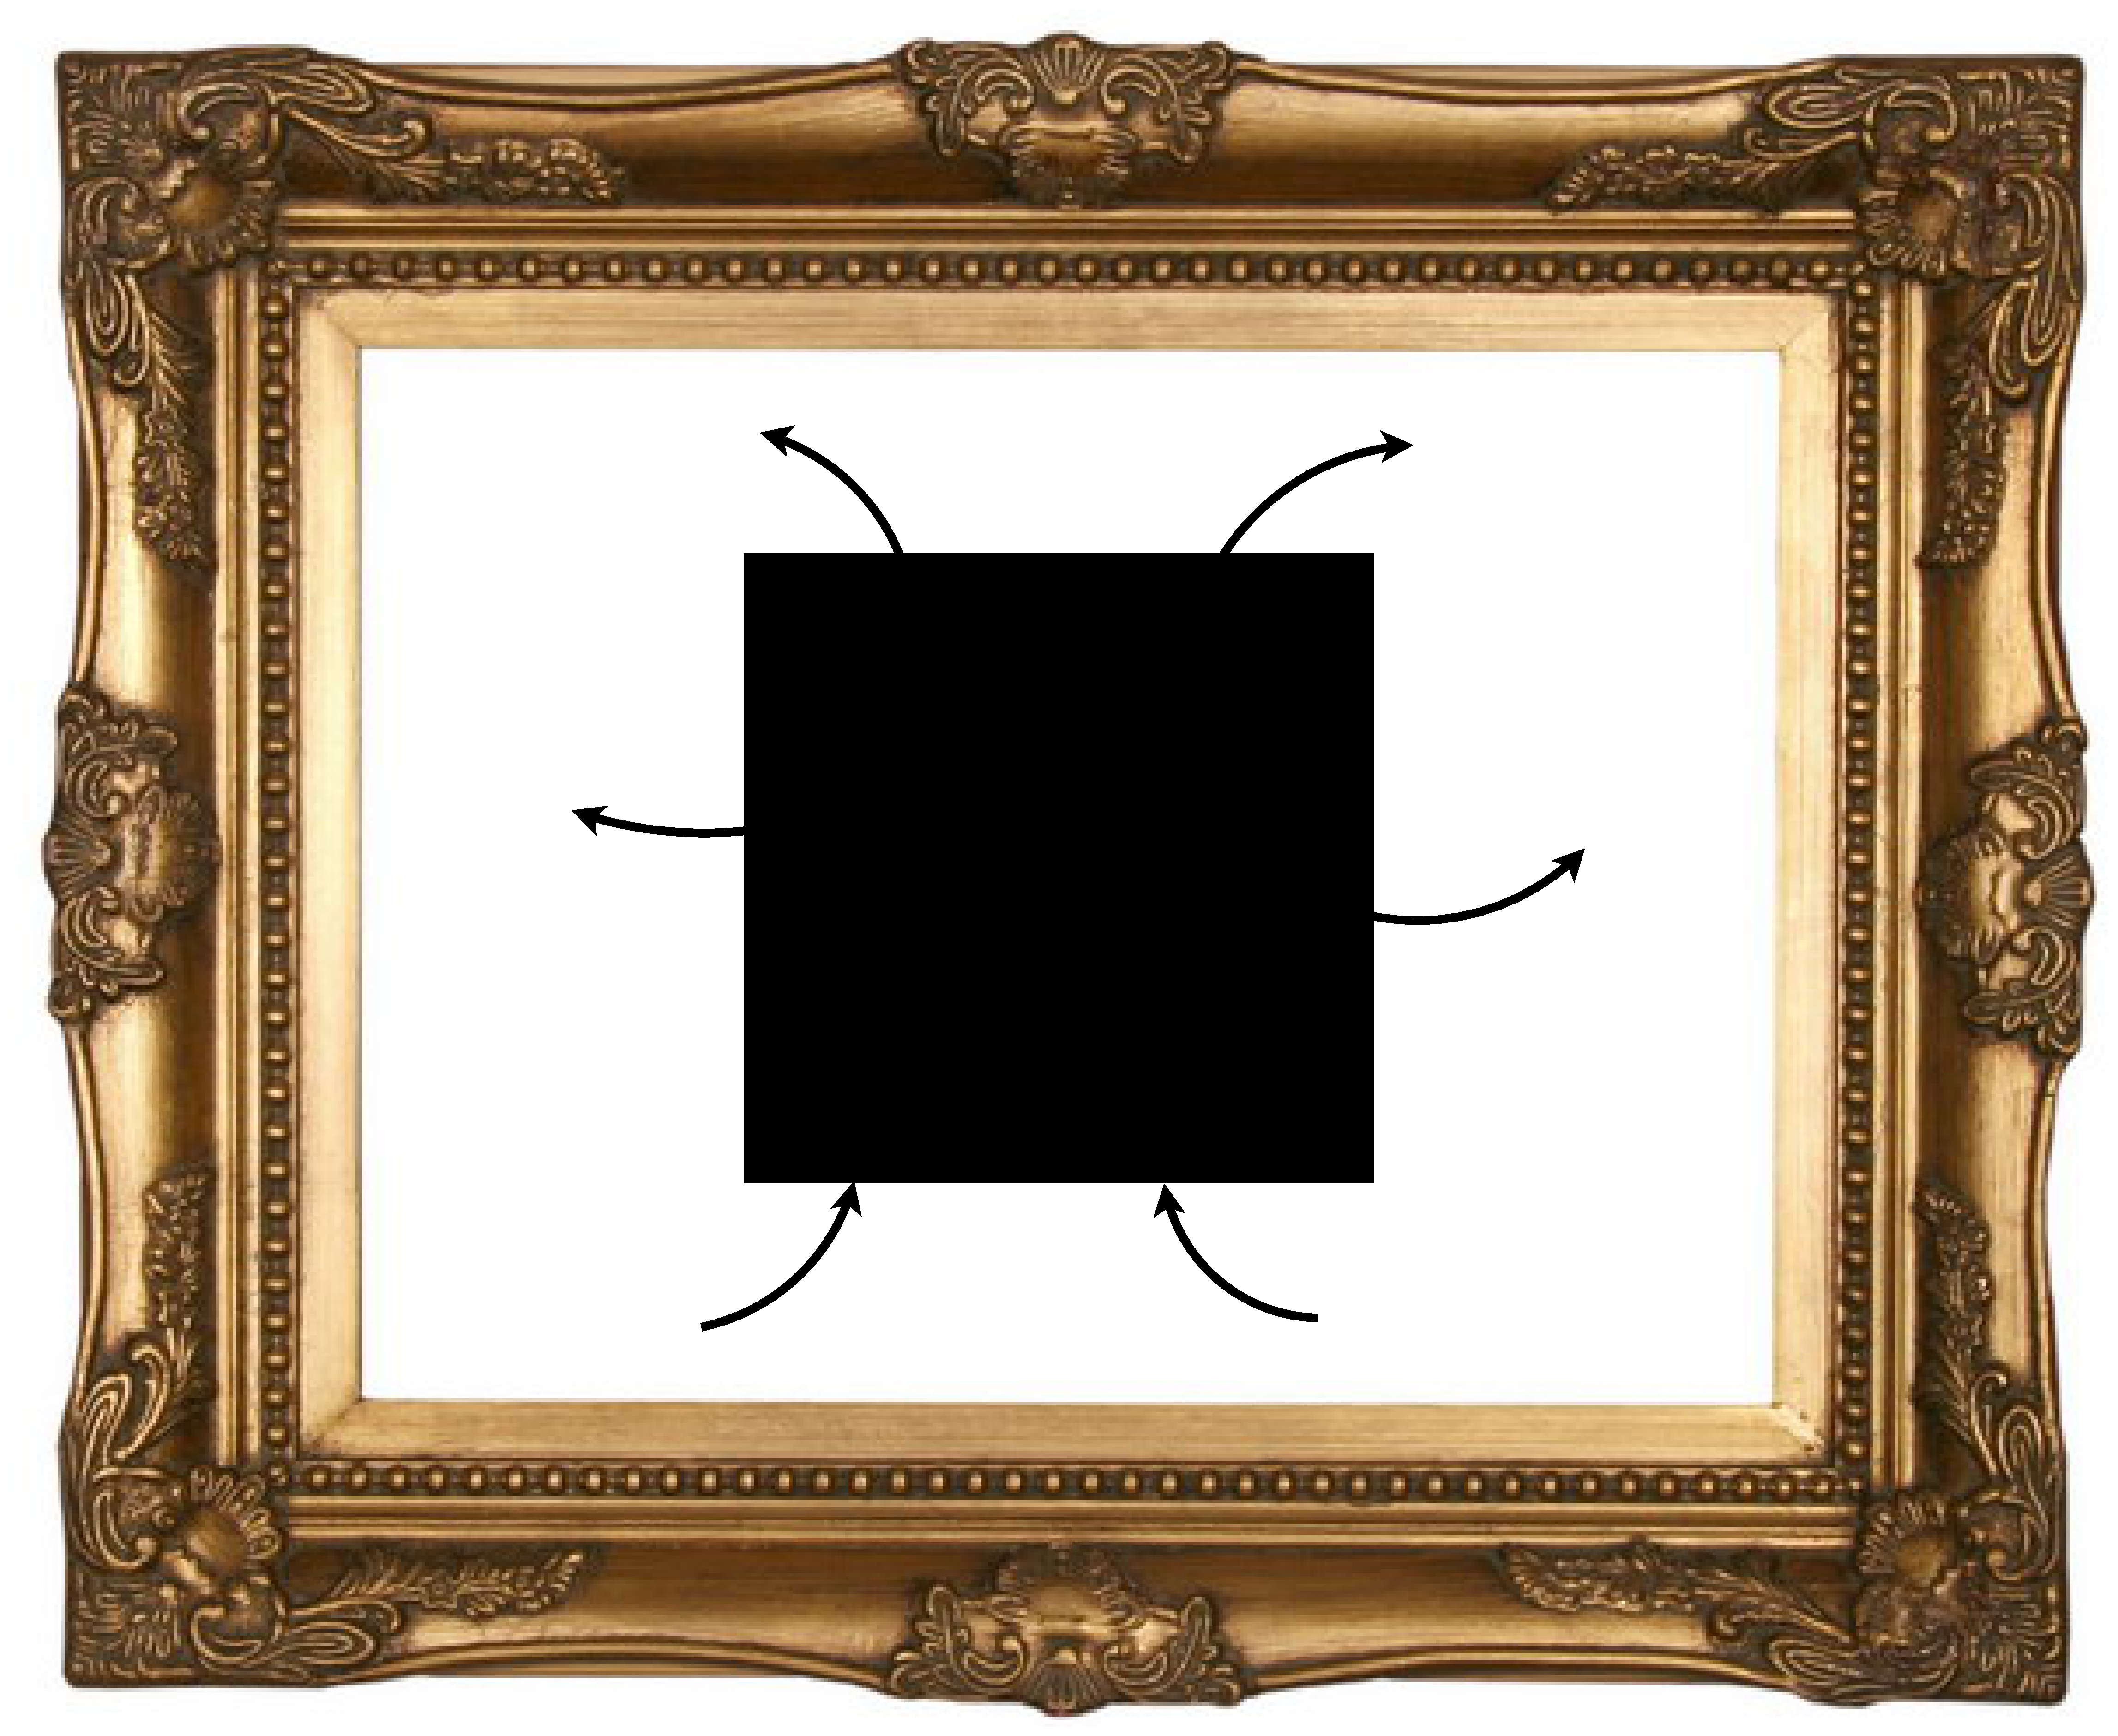
\includegraphics[scale=0.125]{figs/CTBlackBox/CTBlackBox03.eps}}

\onlySlide*{4}{
\includegraphics[scale=0.125]{figs/CTBlackBox/CTBlackBox04.eps}}

\onlySlide*{5}{
\includegraphics[scale=0.125]{figs/CTBlackBox/CTBlackBox05.eps}}

\onlySlide*{6}{
\includegraphics[scale=0.125]{figs/CTBlackBox/CTBlackBox06.eps}}
\end{center}
\end{slide}}







% FR Pu SE and FR Am SE
\begin{slide}{3D Table for FR Pu SE \& FR Am SE}
\begin{center}
\tiny
\begin{tabular}{|c||c|c|c||c|}
\hline
\multicolumn{5}{|c|}{Slice for 0.9 $<$ \texttt{FR\_SE\_AM} $<$ 0.99}\\
\hline
\texttt{FR\_SE\_PU} & $[0.9, 0.99]$ & $[0.99, 0.999]$& $[0.999, 0.9999]$&\\
\hline
$10^4 <$ \texttt{Capacity} $< 10^5$&$426$&$41$&$27$&$494$\\
\hline
$10^5 <$ \texttt{Capacity} $< 10^6$&$10818$&$9937$&$9458$&$30213$\\
\hline
$10^6 <$ \texttt{Capacity} $< 10^7$&$270$&$1694$&$2191$&$4155$\\
\hline
$10^7 <$ \texttt{Capacity} $< 10^8$&$0$&$0$&$2$&$2$\\
\hline
&$11514$&$11672$&$11678$&$34864$\\
\hline
\hline
\multicolumn{5}{|c|}{Slice for 0.99 $<$ \texttt{FR\_SE\_AM} $<$ 0.999}\\
\hline
\texttt{FR\_SE\_PU} & $[0.9, 0.99]$ & $[0.99, 0.999]$& $[0.999, 0.9999]$&\\
\hline
$10^4 <$ \texttt{Capacity} $< 10^5$&$162$&$0$&$0$&$162$\\
\hline
$10^5 <$ \texttt{Capacity} $< 10^6$&$10425$&$6114$&$5356$&$21895$\\
\hline
$10^6 <$ \texttt{Capacity} $< 10^7$&$1105$&$5455$&$6201$&$12761$\\
\hline
$10^7 <$ \texttt{Capacity} $< 10^8$&$0$&$34$&$219$&$253$\\
\hline
&$11692$&$11603$&$11776$&$35071$\\
\hline
\end{tabular}
\end{center}
\end{slide}




% FR Pu SE and FR Am SE
\begin{slide}{3D Table for FR Pu SE \& FR Am SE}
\begin{center}
\tiny
\begin{tabular}{|c||c|c|c||c|}
\hline
\multicolumn{5}{|c|}{Slice for 0.999 $<$ \texttt{FR\_SE\_AM} $<$ 0.9999}\\
\hline
\texttt{FR\_SE\_PU} & $[0.9, 0.99]$ & $[0.99, 0.999]$& $[0.999, 0.9999]$&\\
\hline
$10^4 <$ \texttt{Capacity} $< 10^5$&$151$&$2$&$0$&$153$\\
\hline
$10^5 <$ \texttt{Capacity} $< 10^6$&$10267$&$5560$&$4655$&$20482$\\
\hline
$10^6 <$ \texttt{Capacity} $< 10^7$&$1273$&$5946$&$6038$&$13257$\\
\hline
$10^7 <$ \texttt{Capacity} $< 10^8$&$0$&$179$&$832$&$1011$\\
\hline
&$11691$&$11687$&$11525$&$34903$\\
\hline
\hline
\multicolumn{5}{|c|}{Aggregation over \texttt{FR\_SE\_AM}}\\
\hline
\texttt{FR\_SE\_PU} & $[0.9, 0.99]$ & $[0.99, 0.999]$& $[0.999, 0.9999]$&\\
\hline
$10^4 <$ \texttt{Capacity} $< 10^5$&$739$&$43$&$27$&$809$\\
\hline
$10^5 <$ \texttt{Capacity} $< 10^6$&$31510$&$21611$&$19469$&$72590$\\
\hline
$10^6 <$ \texttt{Capacity} $< 10^7$&$2648$&$13095$&$14430$&$30173$\\
\hline
$10^7 <$ \texttt{Capacity} $< 10^8$&$0$&$213$&$1053$&$1266$\\
\hline
&$34897$&$34962$&$34979$&$104838$\\
\hline
\end{tabular}
\end{center}
\end{slide}





% 2D Contingency Table Statistics
\overlays{2}{
\begin{slide}{2D Contingency Table Statistics}
\FromSlide{1}
The primary measure of the \textit{strength of association} in 2D 
is the \emph{Uncertainty Coefficient} $U(x|R)$.
\[ U(x|R) = \frac{I(R,x)}{H(x)} \]

\FromSlide{2}
This metric has the following useful properties:
\begin{enumerate}
    \item Defined on the range $[0, 1]$.
    \item $U(x|R) = 0$ implies that $I(R,x) = 0$, the parameter
        is unassociated with the response.
    \item $U(x|R) = 1$ requires that $I(R,x) = H(x)$.  This implies that
        the system response $R(x)$ is solely determined by $x$.
\end{enumerate}
\end{slide}}





% 3D Contingency Table Statistics
\overlays{4}{
\begin{slide}{3D Contingency Table Statistics}
\FromSlide{1}
\begin{itemize}
    \item While $U(x,y|R)$ is roughly equivalent to the concept of \textit{mutual} \textit{sensitivity},
        3D tables should allow for an information theoretic parallel to \textit{\underline{covariance}}.

\FromSlide{2}
    \item In general for contingency tables covariance is not well defined, however here there is 
        the special stochastic situation where $x$ and $y$ are known \textit{a priori} to be independent of $R$.

\FromSlide{3}
    \item Therefore, the following new coefficient of variation metric is proposed:

\FromSlide{4}
        \begin{itemize}
            \item $c_v(x|y|R)$ is the \textit{`sensitivity of sensitivity'}, or how much an input 
                affects the response of another input.
        \end{itemize}

\FromSlide{1}
\end{itemize}
\end{slide}}





% 3D Contingency Table Statistics
\overlays{3}{
\begin{slide}{3D Contingency Table Statistics}
\FromSlide{1}
First, define:
\[ U(x|R)|y = \left\{ \left.U(x|R)\right|_{l_0}^{l_1}, \left.U(x|R)\right|_{l_1}^{l_2}, \ldots \left.U(x|R)\right|_{l_{C-1}}^{l_C}  \right\} \]

\FromSlide{2}
Then the coefficient of variation is,
\[ c_v(U(x|R)|y) = \frac{\sigma(U(x|R)|y)}{\mu(U(x|R)|y)} \]

\FromSlide{3}
Finally, the symmetric $c_v$ is set as:
\[ c_v(x|y|R) = \frac{1}{2} \left(c_v(U(x|R)|y) + c_v(U(y|R)|x)\right) \]
\end{slide}}



% 3D Contingency Table Statistics
\begin{slide}{3D Contingency Table Statistics}
\vspace{1.5cm}
Thus, $c_v(x|y|R)$ has the following properties:
\begin{enumerate}
    \item Defined on the range $[0, 1]$ since $0 \le U \le 1$.
    \item $c_v = 0$ implies that $\sigma = 0$, which indicates that $U(x|R)$
        shows no association with $y$.  Thus there are no covariant effects observed.
    \item $c_v = 1$ indicates that $\sigma = \mu$.  This connotes
        that the value of $x$ solely governs the response $R$ from $y$.
\end{enumerate}
\end{slide}





% $c_v(x|y|R)$ Parameter Pair Rankings
\begin{slide}{$c_v(x|y|R)$ Parameter Pair Rankings}
\begin{center}
\tiny
\begin{tabular}{|r|l|l|c|}
\hline
\textbf{Rank}&\textbf{$x$}&\textbf{$y$}&\textbf{$c_v(x|y|R)$}\\
\hline
1&\texttt{FR\_SE\_AM}&\texttt{HLW\_Storage\_Time}&0.02318\\
\hline
2&\texttt{FR\_SE\_AM}&\texttt{FR\_SE\_PU}&0.02316\\
\hline
3&\texttt{HLW\_Storage\_Time}&\texttt{LWR\_UF\_Storage\_Time}&0.01557\\
\hline
4&\texttt{FR\_SE\_PU}&\texttt{HLW\_Storage\_Time}&0.01556\\
\hline
5&\texttt{HLW\_Storage\_Time}&\texttt{LWR\_SE\_PU}&0.01155\\
\hline
6&\texttt{FR\_SE\_AM}&\texttt{FR\_TRU\_CR}&0.01061\\
\hline
7&\texttt{FR\_SE\_PU}&\texttt{LWR\_UF\_Storage\_Time}&0.008192\\
\hline
8&\texttt{FR\_SE\_PU}&\texttt{LWR\_SE\_PU}&0.008\\
\hline
9&\texttt{FR\_BUd}&\texttt{FR\_SE\_AM}&0.007716\\
\hline
10&\texttt{Ambient\_Temp}&\texttt{FR\_SE\_PU}&0.007489\\
\hline
11&\texttt{Ambient\_Temp}&\texttt{HLW\_Storage\_Time}&0.007367\\
\hline
12&\texttt{HLW\_Storage\_Time}&\texttt{LWR\_SE\_AM}&0.007248\\
\hline
13&\texttt{Ambient\_Temp}&\texttt{FR\_SE\_CS}&0.007235\\
\hline
14&\texttt{Ambient\_Temp}&\texttt{LWR\_Fuel2Mod}&0.007066\\
\hline
%15&\texttt{Ambient\_Temp}&\texttt{Heat\_Loss\_Factor}&0.007044\\
%\hline
\end{tabular}
\end{center}
\end{slide}






% Parameter Pair Example
\begin{slide}{Parameter Pair Example}
\begin{center}
\begin{figure}
\caption{Total \& Top Contributors to Decay Heat [Watts/kg] of HLW for (\texttt{FR\_SE\_AM}, \texttt{FR\_SE\_PU}).}
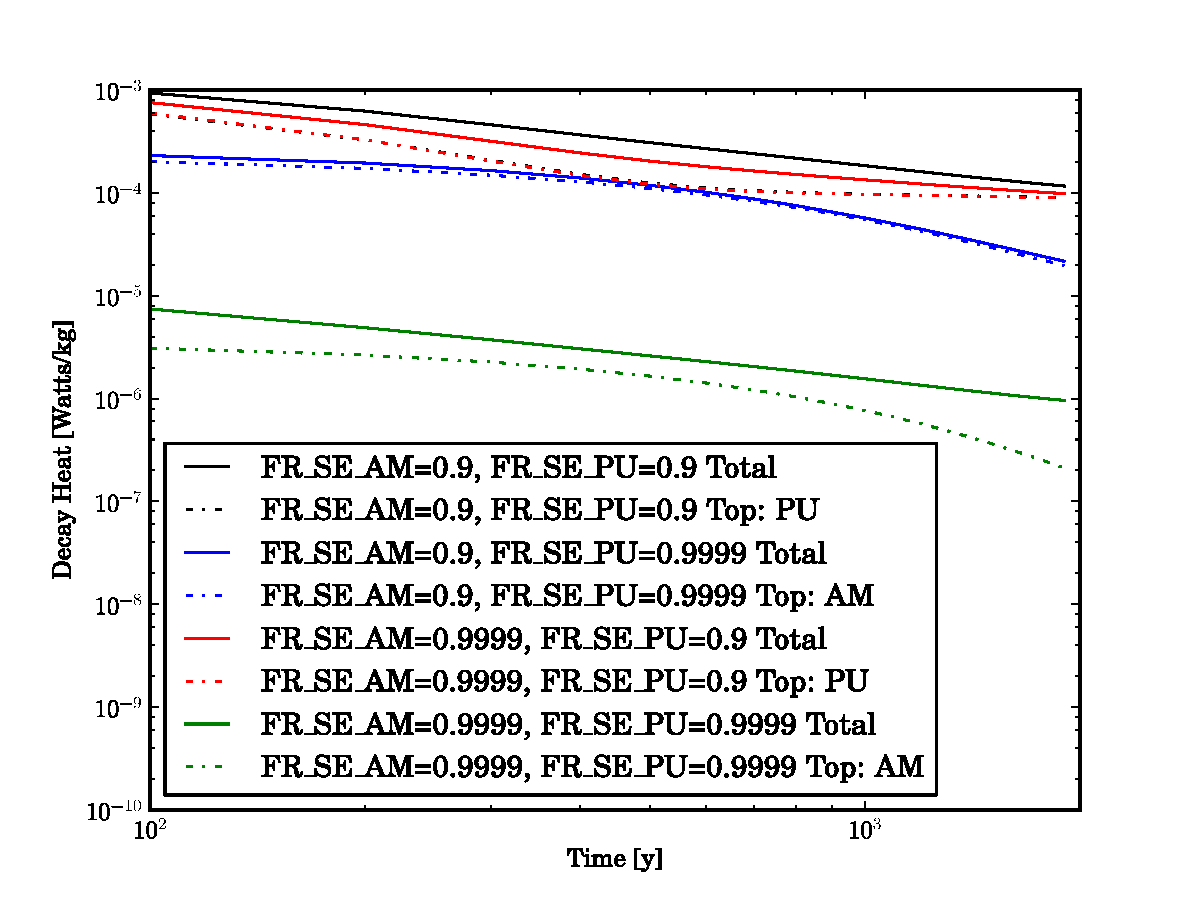
\includegraphics[scale=0.375]{figs/FR_SE_AM_and_FR_SE_PU_Decay_Heat.eps}
\end{figure}
\end{center}
\end{slide}





% Conclusions
\overlays{4}{
\begin{slide}{Conclusions}
\FromSlide{1}
\begin{itemize}
    \item The modeling suite presented here is a new, multi-scale approach to 
    fuel cycle system design.

\FromSlide{2}
    \vspace{0.5cm}
    \item In fact, the speed and fidelity at which the underlying models operate 
        \emph{enables} the new fuel cycle analytics which were demonstrated.

\FromSlide{3}
    \vspace{0.5cm}
    \item Moreover, the $c_v$ metric correctly ranks parameter pairs for with
        an intuitively high covariance.

\FromSlide{4}
    \vspace{0.5cm}
    \item Future work may include tighter integration with the repository model, 
    categorical fuel cycle analysis, and the exploration of alternative metrics.

\FromSlide{1}
\end{itemize}
\end{slide}}







% Questions
\begin{slide}{Questions}
? ? ? ? ? ? ? ? ? ? ? ? ? ? ? ? ? ? ? ? ? ? ? ? ? ? ? ? ? ? ? 
? ? ? ? ? ? ? ? ? ? ? ? ? ? ? ? ? ? ? ? ? ? ? ? ? ? ? ? ? ? ? 
? ? ? ? ? ? ? ? ? ? ? ? ? ? ? ? ? ? ? ? ? ? ? ? ? ? ? ? ? ? ? 
? ? ? ? ? ? ? ? ? ? ? ? ? ? ? ? ? ? ? ? ? ? ? ? ? ? ? ? ? ? ? 
? ? ? ? ? ? ? ? ? ? ? ? ? ? ? ? ? ? ? ? ? ? ? ? ? ? ? ? ? ? ? 
? ? ? ? ? ? ? ? ? ? ? ? ? ? ? ? ? ? ? ? ? ? ? ? ? ? ? ? ? ? ? 
? ? ? ? ? ? ? ? ? ? ? ? ? ? ? ? ? ? ? ? ? ? ? ? ? ? ? ? ? ? ? 
? ? ? ? ? ? ? ? ? ? ? ? ? ? ? ? ? ? ? ? ? ? ? ? ? ? ? ? ? ? ? 
? ? ? ? ? ? ? ? ? ? ? ? ? ? ? ? ? ? ? ? ? ? ? ? ? ? ? ? ? ? ? 
? ? ? ? ? ? ? ? ? ? ? ? ? ? ? ? ? ? ? ? ? ? ? ? ? ? ? ? ? ? ? 
? ? ? ? ? ? ? ? ? ? ? ? ? ? ? ? ? ? ? ? ? ? ? ? ? ? ? ? ? ? ? 
? ? ? ? ? ? ? ? ? ? ? ? ? ? ? ? ? ? ? ? ? ? ? ? ? ? ? ? ? ? ? 
? ? ? ? ? ? ? ? ? ? ? ? ? ? ? ? ? ?
\end{slide}

\begin{slide}{Bibliography}
\tiny
\begin{enumerate}
    \item \fullcite{Scopatz2009}
    \item \fullcite{Li2010a}
    \item \fullcite{NEA-5990}
    \item \fullcite{Scopatz2010a}
    \item \fullcite{Takano1994}
    \item \fullcite{Press2007c}
    \item \fullcite{ENDF}
    \item \fullcite{Croff2002}
\end{enumerate}
\end{slide}

\end{document}
